\documentclass[11pt]{article}
\usepackage{float}
\usepackage{fullpage}
\usepackage{amssymb}
\usepackage{amsthm}
\usepackage{color}
\usepackage{enumerate}
\usepackage{amsmath}
\usepackage{graphicx}
\usepackage[margin=0.8in]{geometry}
\usepackage{listings}
\usepackage{framed}
\lstset{
	language=C,
	basicstyle=\scriptsize\ttfamily,
	commentstyle=\ttfamily\color{green},
	numbers=left,
	numberstyle=\ttfamily\color{blue}\footnotesize,
	stepnumber=1,
	numbersep=5pt,
	backgroundcolor=\color{white},
	showspaces=false,
	showstringspaces=false,
	showtabs=false,
	frame=single,
	tabsize=2,
	captionpos=b,
	breaklines=true,
	breakatwhitespace=false,
	title=\lstname,
	escapeinside={},
	keywordstyle={},
	morekeywords={}
}

\setcounter{secnumdepth}{0}

\begin{document}

\title{Report: ARM11 Project \\ Group 8}
\author{Elliot Grenwood, Elyas Addo, Florian Emile, Nana Asiedu-Ampem}

\maketitle

\section{Introduction}
This report covers the completion of Group 8's ARM11 Project, specifically Parts II - IV: Assembler; General Purpose Input/Output on a Raspberry Pi; our chosen extension. The assembler program, like the emulator, is written in C. Part of the extension is also written in C, and the other part in the ARM11 assembly language. In this report we will also discuss the organisation and communication of the group.

\section{Part II - Assembler}

Our assembler can be split into 6 subtasks:\newline

1. Input/output setup with \verb|setUpIO()| in \texttt{assemble.c} which simply sets the pointer
to the input and output files.\newline

2. Breaking up the input file with \verb|tokenise()| in \texttt{tokenise.c}; an array of tokens is created where a token is composed of two fields - the original string and the token type (e.g. \texttt{LABEL}).\newline

3. Mapping all of the labels in the program to their addresses using \verb|resolveLabelAddresses()| in \texttt{assemble.c};\newline

4. Parsing in the input file with \verb|parseProgram()| in \texttt{parse.c}. Since different instructions require different components (flags, arguments, e.t.c.), parse functions have been written to cater for all instruction types. Each parse function computes the arguments to pass in the generate functions (below) by accessing the symbol tables that links the "word" to the matching number and by
computing the flags that are set.\newline

5. Generating the instruction in binary for each type of opcode using generate
functions (different for every type of opcode) all in \texttt{generate.c.}\newline

6. Writing the binary instruction to the output file using \verb|ouputData()| in \texttt{assemble.c}.\newline

Using assembly files in a provided testsuite, the \texttt{./assemble} outputs were compared to the expected outputs to ensure the program function correctly. We also built files for testing data structures, such as the queue - this ensured we knew this unit of the program was working as we wanted to, affording us the opportunity to use it's functions freely in our program.

\section{Part III - GPIO}
%nana for emulate, no change for assembler, testing - flashes\newline

We added constants that contain the GPIO set/clear area addresses that will be used to alter their outputs. Three more constants were made to contain the GPIO status addresses that modify the state of each pin.  Memory was allocated for all five of the addresses. The emulator had to be updated to allow these addresses to be modify. This was done by adding functionality to the functions that access memory locations. If these special memory address are being accessed (e.g. 0x2020 0004) then our program alters their respective memory locations rather than the allocated RAM memory used to store the instructions.

\section{Part IV - Extension}
Our chosen extension has 4 parts: changing the functionality of \texttt{mov r15, r14} to allow returns from function calls; allowing the use of comments in an assembler file being passed into our assembly program; creating a 3 bit binary counter in assembly language; creating a IR-based counter. \newline

% talk about the fact we built it up from a flashing LED, to a binary counter, to an IR counter

% all have description, design, problems, testing

\subsection{Comments}
The ability to write comments alongside instructions is a useful feature. It can improve the clarity of assembly code which allows for easier maintainance. Comments begin with a semi-colon and finish at the end of the line. They can be placed either on an empty line or at the end of an instruction. For a new-line and end-of-line comments there are 3 types to test for: a blank comment with no text (e.g. \texttt{;}), a comment with no spaces at the start (e.g. \texttt{;comment}), a comment with spaces after the start (e.g. \texttt{; comment}).\newline

\noindent Since comments only exist in an assembly file, only the assembler program had to be edited. The \verb|tokenise()| function was amended to check for a \texttt{;} at the beginning of a token, and if one is found, start reading the next line. Although the comment update was implemented by a member of the group who didn't work on the tokeniser, change was easily made due to the clarity of the original design.\newline

\noindent Figure 1 below shows the \texttt{./emulate} output for the \texttt{commentTest} program assembled with and without the comments. We also used our assembler on the original test suite to ensure the feature didn't affect any other element of the program.
\lstinputlisting{commentTest.s}

\begin{figure}[H]
	\centering
	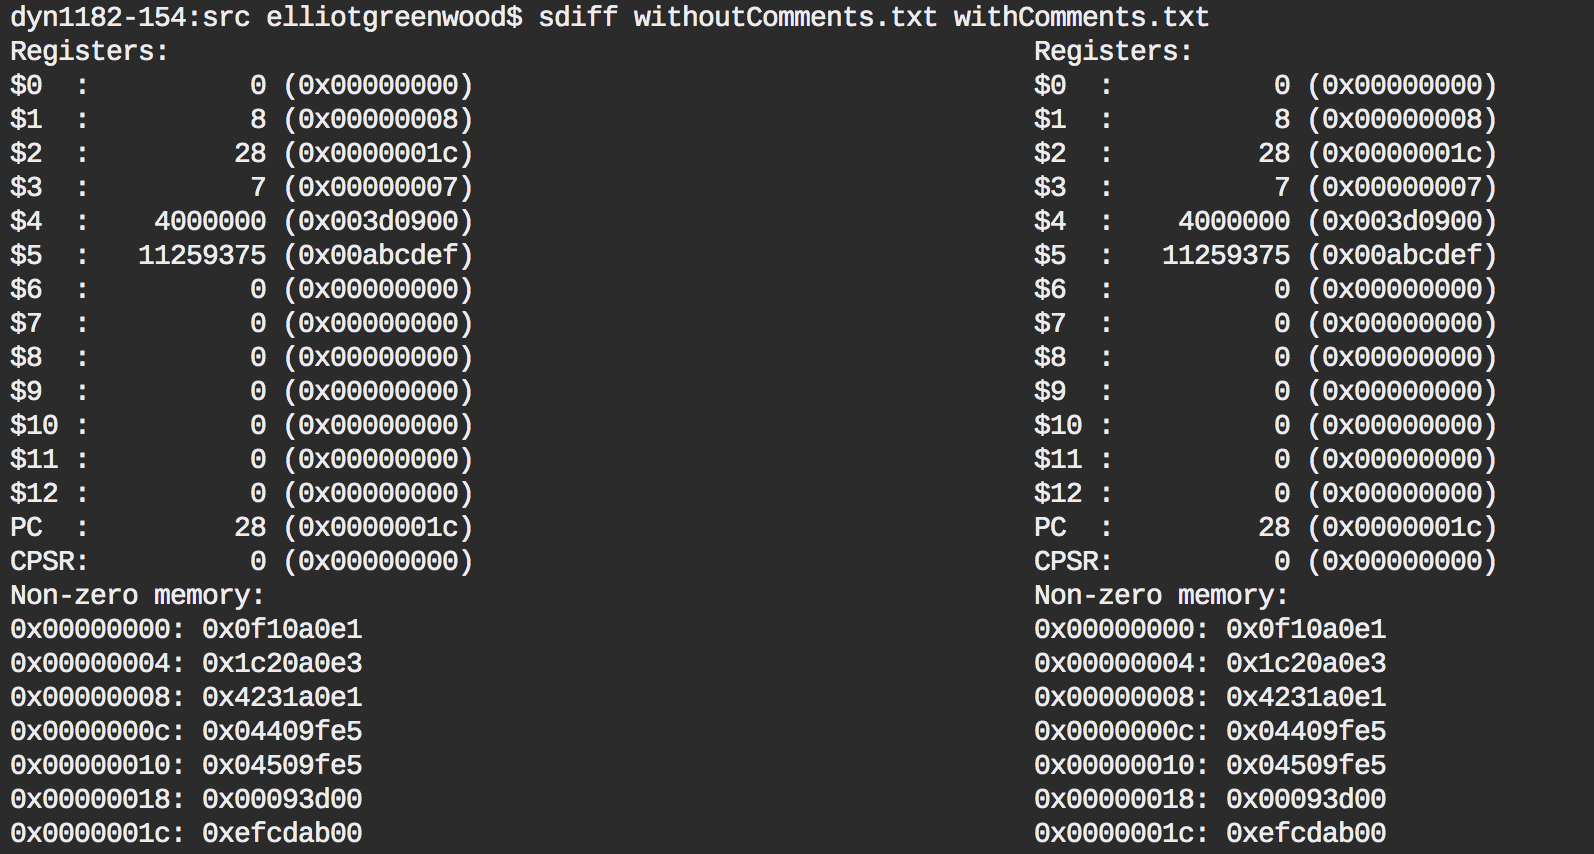
\includegraphics[scale = 0.5]{commentTest}
	\caption{Abhinav Gandhi taught me how to do this}
\end{figure}

\subsection{3 Bit Binary Counter}
\subsection{Implementing \texttt{mov r15, rn}}
In order to use functions, a program can create its own stack structure in memory. This allows the program to store the derived return address and then branch to a function. However, in order to return from a function the PC must store the return address whilst maintaining the pipeline effect. The ARM11 architecture already has a \texttt{mov PC, rn} command which braches automatically so \texttt{./assemble} needs no changing. However, to test the function we have improved the \texttt{mov} instruction in the emulator to allow the PC to store in a chosen address and then branch immediately. again this was very little challenge as it simply involved a small if statement.
\subsection{IR-Based Counter}

  - all have description, design, problems, testing

\section{Reflection of working in a group}
\subsection{Elliot Greenwood}
\subsection{Elyas Addo}
\subsection{Florian Emile}

I thought that the most challenging part of the project would have been writing
in assembly. However coding the assembler in C was the trickiest as C was new to
me and the tasks in assembly were straightforward. I had to get used to drawing
flowcharts and writing pseudo codes for part II as it made my task easier.

I found my programming skills were not on par with those of my team members. I
verified if I understood the concepts before coding. I kept my team leader
informed of my progress as I made it easier for him to help me. When I was
working on a task with someone, I was always open to his suggestions since we
can find what we think is the best solution faster.

In a different team, I would keep my team (especially team leader) informed of
my progress in the task at hand I would also like to be more independent when I
am assigned an individual task.

\subsection{Nana Asiedu-Ampem}
\subsection{Group Reflection}

\end{document}
